%!TEX root = main.tex
% \section{Motivations and Opportunities}
\section{Challeges and Motivations}
\label{sec:cam}
\subsection{Memory Imbalance in Pipeline Parallelism}
% Pipeline parallelism partitions the model across multiple GPUs
% for parallel training to accommodate larger models when
% the memory of a single GPU is insufficient to hold the model training.
% However, existing pipeline parallelism methods mainly consider the balance of computation
% across different stages, while neglecting the very uneven memory usage among stages.
% This leads to a huge waste of GPU memory,
% which seems to contradict the original intention of training larger models.
Pipeline parallelism is designed to fit
the large model's training to multiple devices
when the memory of single device is not able to accommodate it.
However, we have observed huge memory waste due to the memory imbalance across pipeline stages,
which seems in contrary to the original intention.
To illustrate this memory imbalance, we conduct a benchmark test on the peak memory usage of
each stage on the GPipe and PipeDream.
The test was conducted on a server equipped with 8 A100 GPUs (40 GB),
with the pipeline stages of GPipe and PipeDream being 4 and 8, respectively.
\begin{figure*}[t]
  \centering
  \begin{minipage}[t]{0.33\linewidth}
    \centering
    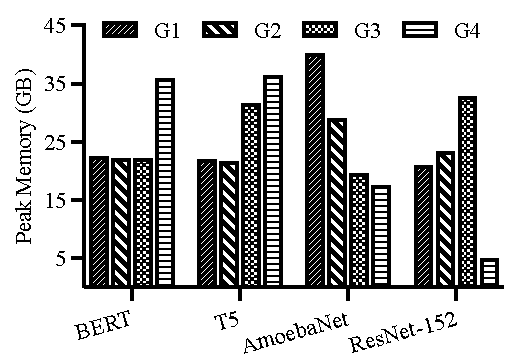
\includegraphics[width=0.95\linewidth]{GPipe-4GPUs.pdf}
    \caption{GPipe-4GPUs}
    \label{fig:gpipe-4gpus}
  \end{minipage}
  \begin{minipage}[t]{0.33\linewidth}
    \centering
    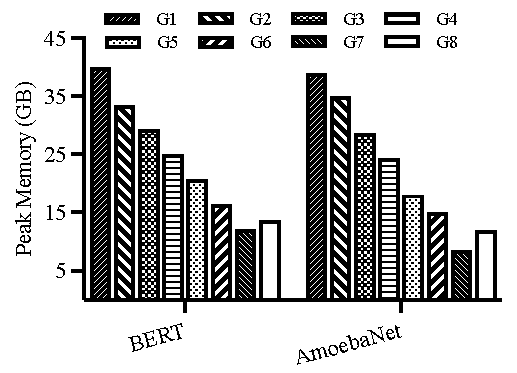
\includegraphics[width=0.95\linewidth]{PipeDream-8GPUs.pdf}
    \caption{PipeDream-8GPUs}
    \label{fig:pd-8gpus}
  \end{minipage}
  \begin{minipage}[t]{0.33\linewidth}
    \centering
    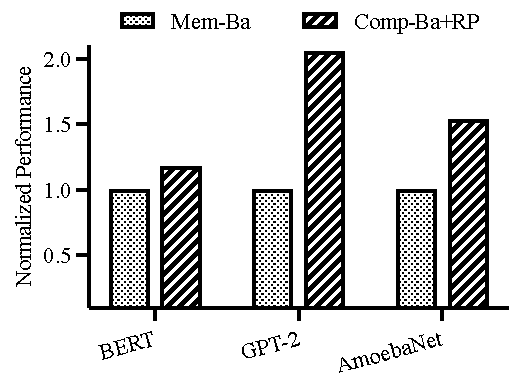
\includegraphics[width=0.95\linewidth]{normalized-perf.pdf}
    \caption{Normalized Performance}
    \label{fig:norm-perf}
  \end{minipage}
  % \caption{Peak Memory Footprint}
  % \label{fig:peakmem}
\end{figure*}


The benchmark results on the GPipe are shown as Figure~\ref{fig:gpipe-4gpus},
where the G0 to G3 represent the GPU numbers.
It can be seen that for the BERT model,
the peak memory usage of the first three stages are basically the same,
and the peak memory usage of the last stage is 13 GB higher than the previous stages.
This is because BERT is a Transformer-based model built by the encoder,
in which the computation time and memory usage of the hidden layers are basically consistent,
resulting in very balanced memory usage in the first three stages.
However, the last stage has additional loss calculations
and some subsequent processing functions,
and the peak memory usage for training generally occurs
at the beginning of the backward computation,
so the memory usage of the last stage increases significantly.
This phenomenon also exists for T5, which is also a Transformer-based model.
The difference is that T5 is built by the encoder and decoder,
which results in a higher peak memory usage in the third stage.
% so when the model partitioning is aimed at computational balance,
% it leads to higher memory usage in the third stage.
However, the ratio of computation to memory usage
of different layers is no longer consistent in the CNN models.
For example, the convolutional layers usually have longer computation time,
while the fully connected layers consume more memory.
% resulting in layers that occupy only a
% small amount of memory but generate a lot of computation time.
This phenomenon is particularly evident in ResNet-152,
where the last stage accounts for about 1/4 of the total computation time,
but the memory footprint only accounts for about 5 GB,
a difference of more than 27 GB compared to the third stage with the most memory occupied.
If we use the maximizes peak memory usage across all stages as the GPU capacity baseline,
then there is nearly 40\% and 34\% of the GPU memory wasted in ResNet-152 and AmoebaNet.
% If the peak memory usage in all stages is taken as the benchmark for the total GPU capacity,
% then in ResNet-152, nearly 40\% of the GPU memory is wasted,
% and in the AmoebaNet model, this memory waste ratio is 34\%.

In the synchronous pipeline parallelism,
the memory imbalance across stages is mainly
due to the uneven ratio of computation time
to memory usage of different layers in the model.
In the asynchronous pipeline parallelism,
in addition to the above reason,
the inconsistency in the number of copies of model parameters,
activation memory, and gradients required by each stage will
further exacerbate this memory usage imbalance.
% If in a synchronous pipeline parallel system like GPipe,
% the imbalance of memory usage between stages is mainly
% due to the uneven ratio of computation to memory usage between layers in the model,
% then in an asynchronous pipeline parallel system like PipeDream, in addition to the above reason,
% the inconsistency in the number of copies of model parameters, activation memory,
% and gradients required by each stage will further exacerbate this phenomenon of uneven memory usage.
The benchmark results on the PipeDream are shown in Figure~\ref{fig:pd-8gpus}.
It can be seen that the peak memory usage of the first stage
reaches 40 GB while the smallest peak memory usage is only 12 GB in BERT.
% of model parameters, activation memory, and gradient memory,
% In the BERT model, because the first stage needs to store 8 copies
% of model parameters, activation memory, and gradient memory,
% its peak memory usage is the highest, reaching 40 GB,
% while the stage with the least memory usage is the penultimate stage,
% with only 12 GB of memory usage.
The memory waste ratio of BERT in GPipe is about 28\%,
while this ratio has exceeded 40\% in PipeDream.
% while in the 8-GPU PipeDream, the memory waste ratio has exceeded 40\%,
Furthermore, the memory waste ratio of AmoebaNet also decreased
by nearly 10\% compared to the result in GPipe.
As a result, whether it is synchronous or asynchronous pipeline parallelism,
a large amount of GPU memory is wasted,
limiting the scale of the model that can be supported to the stage with the maximum memory usage,
even though there is still a lot of free memory on the other GPUs.

% Although pipeline parallelism are designed to fit the large model's training to multiple devices
% when single device's memory is not able to accommodate it,
% we have observed huge memory waste due to the memory imbalance across pipeline stages,
% which seems in contrary to the original intention.
% There are mainly two reasones.
% Firstly, the training performance has always been the first priority for pipeline parallelism in previous work.
% Therefore, the most important factor to the training performance is the computation balance across stages,
% since a straggeler stage will slow down the overall training speed of pipeline parallelism.
% In such way, the memory usage balance across stages is ignored when partitioning the model,
% and this memory imbalance is especially obvious for those models whose layers have a big variance
% of the computation time and memory consumption ratio,
% e.g., convolutional layers usually have longer computation time
% but fully connected layers usually consume much more memory.
% Secondly, for the asynchronous pipeline parallelism, which though shows great device utilization,
% it also exacerbates the memory imbalance across stages.
% It's because the former stage needs to store more versions of the model parameters
% and activation/gradient memory for different micro-batches.
% Based on the memory imbalance caused by the first reason,
% this can amplify the existing memory imbalance.

% We perform a benchmark of the peak memory footprint of each stage on
% synchronous PP (GPipe) and asynchronous PP (PipeDream),
% and the results are shown as Figure~\ref{fig:peakmem}.
% The benchmark was performed on a server equipped with 8 A100 GPUs (40~GB memory).

\subsection{Computation Balance}
% In previous works, they perform the model partition in PP at a coarse granularity
% especially for the large language model. A major reason is that .
% For example, the Bert model is built by the basic layer block, \texttt{BertLayer}
% in HuggingFace's Transformers~\cite{wolfHuggingFaceTransformersStateoftheart2020}.
% However, a single layer block can contains lots of \emph{atomic operations} in the
% underlying framework, such as PyTorch.
Based on the above discussion, it can be seen that
focusing on the balance of computation across stages
can easily lead to imbalanced memory usage among stages, and vice versa.
% However, simply balancing the memory usage between stages
% can easily result in a large difference in computation time between stages,
% thereby affecting the overall training performance.
At the same time, due to the existence of memory optimization methods,
i.e., the memory swapping and recomputation,
% which are mainstream and universal techniques,
a problem is when the GPU memory has oversubscribed
after a model is partitioned by computational balance,
whether to partition the model to be more memory balanced to meet the memory requirements,
or to leverage memory optimization methods to optimize
the stages that exceed the GPU memory capacity.
% a problem is whether to partition a pipeline parallelism,
% which exceeds the GPU memory capacity after being divided according to computational balance,
% to be more memory-balanced to meet the memory capacity requirements,
% or to use memory optimization methods to optimize
% the parts that exceed the GPU memory capacity.
It is hard to know which of these two methods is superior in terms of training performance.
Therefore, we implement two simple partitioning methods in PipeDream for performance comparison.
The first is memory-balance partition (Mem-ba) while the second
is compute-balance in conjunction with recomputation (Comp-ba+RP).
Both of them can achieve comparble maximum batch size
and the communication cost does not affect the training performance.


% To simply verify the above issues,
% we implements two partitioning methods in PipeDream to compares their performance.
% The first is to partition the model so that the GPU memory usage between stages of the pipeline is basically balanced.
% The second method is to partition the model so that the computation time between stages of the pipeline is basically balanced,
% and use recomputation to reduce the GPU memory of the stages with more memory occupation.
% After testing the maximum batch size that can be achieved with the first method,
% adjust the recomputation ratio in the second method to also achieve this batch size,
% and compare the training performance of the two methods at this time.
% It should be noted that in the above two model partitions,
% the amount of inter-stage communication is very small and close,
% and will not affect the performance of pipeline parallel training.
% \begin{figure}
%   \centering
%   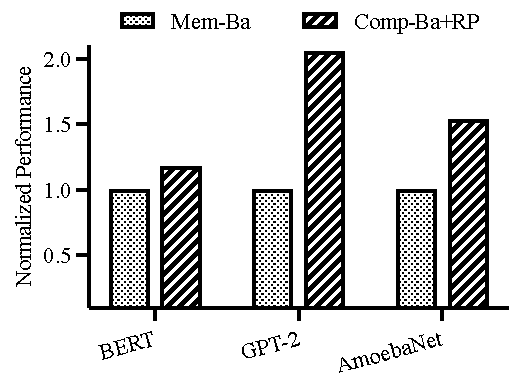
\includegraphics[width=0.85\linewidth]{normalized-perf.pdf}
%   \caption{Normalized Performance}
%   \label{fig:norm-perf}
% \end{figure}

The normalized performance results are shown in Figure~\ref{fig:norm-perf}.
% including performance comparisons of BERT, GPT-2, and AmoebaNet models.
It can be seen that on these three models,
the performance of the second method is always better.
Especially on the GPT-2 model, the training performance of Comp-Ba+RP
is more than 2$\times$ that of memory balance.
This is because there is a huge difference in computation time between the longest and
shortest stages after memory balanced partitioning in GPT-2.
Specifically, the computation time of the fourth stage reaches 286.275 ms,
while that of the first stage is only 29.104 ms, which is nearly a 10$\times$ difference.
This makes the pipeline parallel performance extremely limited by the
excessively long computation time of the fourth stage.
Furthermore, the recomputation in GPT-2 can achieve
large memory reduction with a small amount of recomputation time.
Therefore, in the method of Comp-Ba+RP,
the total computaiton time of the fourth stage is only 145.89 ms,
while the first stage needs to perform more recomputation,
thus making the computation time reach 136.89 ms.
% Therefore, recomputation on the basis of computational balance,
% even though the fourth stage is still the longest in computation time,
% the computation time after adding recomputation is only 145.89 ms,
% while the first stage needs to perform more recomputation,
% thus making the computation time reach 136.89 ms.
It can be seen that the computation time of the fourth stage
is almost half of that in Mem-ba.
% resulting in a very large performance gap between the two.
This is also true for BERT and AmoebaNet,
with gaps of 1.18$\times$ and 1.54$\times$, respectively.
It should be noted that even though the second method
always achieve the better training performance in this benchmark,
it does not mean this is the case in all situations.
The purpose of this section is to illustrate that when comprehensively
considering memory limit, pipeline partitioning, and memory optimization,
achieving optimal pipeline parallel performance is a very complex and difficult problem.

% It should be noted that although the experiments in this section
% all use the method of recomputation to
% achieve better pipeline parallel performance than when balanced for memory,
% this does not mean that this is the case in all situations.
% For example, when it is not necessary to partition memory completely balanced,
% the performance will be significantly improved.
% The purpose of this section is to illustrate that when comprehensively
% considering memory limit, pipeline partitioning, and memory optimization,
% achieving optimal pipeline parallel performance is a very complex and difficult problem.

% \subsection{Layer (block) based Partition}
% In current research, the model partitioning and memory optimization
% of pipeline parallelism are basically carried out
% at the granularity of layers or layer blocks.
% On one hand, this is because existing mainstream models are almost
% all built based on a basic layer block,
% especially in the field of natural language processing,
% models based on the Transformer architecture,
% which are usually integrated into some third-party libraries,
% such as the famous HuggingFace Transformers[99] library.
% It provides tens of thousands of pre-trained Transformer models
% and their model code implementations.
% By abstracting the underlying deep learning systems,
% such as TensorFlow, PyTorch, JAX, etc.,
% it provides reusable model code to different systems,
% greatly reducing the complexity of model training or deployment.
% For example, in the code implementation of the BERT model in this library,
% the middle hidden layers are composed of the basic layer block BertLayer,
% so users can easily build BERT models with different numbers of layers.
% On the other hand, the models provided by users are basically an API interface in these libraries.
% In order to conveniently generate model code for different stages in the subsequent model partitioning,
% existing research needs to expand and rewrite the model structure code at the granularity of layers or layer blocks based on the models provided by users.
% However, such methods are not universal enough in actual production environments,
% such as when the user's model contains custom modules or needs privacy protection and does not want third-party developers to observe the model structure.
% In addition, partitioning and memory management at this relatively coarse granularity easily limits
% the partitionable space and cannot perform memory optimization management at a finer granularity.
% Memory optimization management at a finer granularity, such as the tensor level, has been proven to achieve higher performance in many works[87,100,101].

\subsection{Motivation}
\label{sec:mot}
% In another model parallel approach—tensor parallelism,
% existing research commonly employs deep learning compilation techniques
% to automatically search for tensor parallel splitting strategies
% and generate corresponding model code for different underlying hardware platforms,
% such as GPU, FPGA, ASIC, and other computing platforms.
% Mainstream deep learning systems all have their own set of deep learning compilation frameworks,
% such as XLA in TensorFlow, MindCompiler in MindSpore, and TorchDynamo[102] in PyTorch.
% However, the essence of pipeline parallelism is inter-layer parallelism,
% without modifying the computational logic within operators,
% hence it does not require such a "heavyweight" compilation system as in tensor parallelism.
% Based on this, this chapter first explores the use of lightweight
% deep learning compilation technology for fine-grained testing and analysis of models,
% and can automatically generate model code for different stages under any model partitioning.

We found that the DL compilation technique, like XLA~\cite{sabneXlaCompilingMachine2020} and TorchDynamo~\cite{anselPyTorchFasterMachine2024},
which is extensively adopted in tensor parallelism
for fine-grained analysis and automatic code generation,
is never been used for pipeline parallelism in previous research works.
Furthermore, on the basis of the DL compilation for fine-grained analysis of DL models,
we have discovered two memory usage features during the model training process
for guiding the pipeline parallelism partition.
\begin{figure}[htb]
  \centering
  \subfigure[Activation memory]{
    \centering
    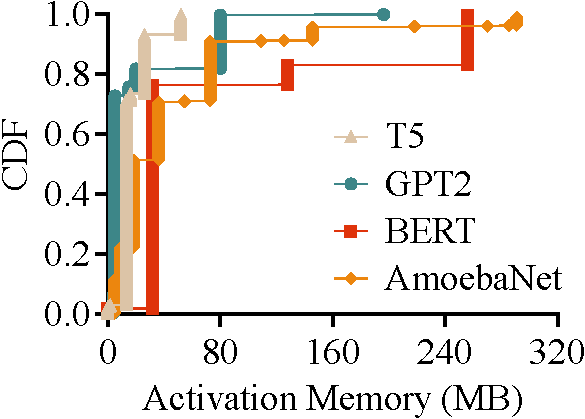
\includegraphics[width=0.47\linewidth]{act-mem-cdf-crop.pdf}
    \label{fig:act-mem-cdf}
  }
  \subfigure[Consumed Memory]{
    \centering
    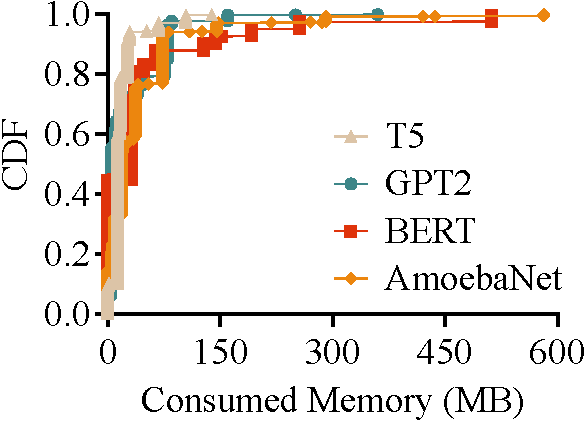
\includegraphics[width=0.47\linewidth]{consumed-mem-cdf-crop.pdf}
    \label{fig:cons-mem-cdf}
  }
  \caption{Memory distribution}
  \label{fig:mem-cdf}
\end{figure}

Firstly, the majority of the activation memory sizes are very small,
which means it's easy to find a small communication volumes between
each stages pair for pipeline partition.
We profile the activations memory size on BERT, T5, GPT-2, and AmoebaNet,
and the results are shown in Figure~\ref{fig:act-mem-cdf}.
Note that for Transformer-based models,
the largest activation memory generally appears at
the output layer of the model,
which means this kind of memory will definitely
in the last stage and won't become the communication targets between pipeline stages.
For AmoebaNet, its largest activation memory (about 580 MB) is
basically the output of some convolutional layers, which only appear 5 times.
Hence, they are omitted in the figures.
It can be seen that in GPT-2, T5, and AmoebaNet,
nodes with activation memory less than 80 MB
account for more than 90\% of the total number of computational nodes.
Especially in T5, except for the final output node,
the activation memory of the other nodes are only about 50 MB.
In BERT, nodes with activation memory not greater
than 128 MB also account for more than 80\% of the total number of nodes.
Although as the pipeline is partitioned, the batch size will increase accordingly.
Assuming that there are 4 stages in the pipeline,
for a 4-times 128 MB memory transfer, i.e., 512 MB,
under the relatively low bandwidth of the PCIe 3.0 $\times$16 link,
the data transfer time will not exceed 40 ms,
which is far less than the computation time.

% On the basis of using compilation methods for fine-grained analysis of models,
% this section has discovered two memory usage characteristics during the model training process.
% The first is that during the forward process of model training,
% although there will be some memory release operations, overall,
% the GPU memory occupation tends to increase,
% which has been proven in many previous research works.
% The second is that the activation memory of a single computational node is usually not very large,
% which means that when performing pipeline partitioning,
% it is easy to make the communication volume between stages relatively small,
% thereby basically not affecting the performance of pipeline parallelism.

% To prove this point, we profile the activation and consumed memory size
% of each node on BERT, T5, GPT-2, and AmoebaNet.
% The selected batch size of each model is to make the peak memory footprint
% closed to the GPU memory capacity (40 GB) as much as possible.
% The results are shown in Figure~\ref{fig:mem-cdf}.
% and adjusted the batch size to make the peak GPU memory occupation
% during training close to the total GPU memory capacity (40 GB).
% The distribution of activation memory sizes at this batch size is shown in Figure~\ref{fig:act-mem-cdf}.

% so when performing pipeline partitioning,
% these memories will only be in the last stage and will not
% become activation memory communicated between different stages of the pipeline,
% hence these large activation memories are omitted in the figure
% (the maximum value in the BERT model is about 900 MB),
% while in the CNN model AmoebaNet, the largest activation memory
% is basically at the output of the convolutional layer, about 580 MB,
% but it only appears 5 times, which can be basically ignored
% compared to the total of more than 1000 computational nodes in the AmoebaNet model.
Secondly, the distribution of the absolute consumed memory sizes are shown as Figure~\ref{fig:cons-mem-cdf}.
% At the same time, this section also counted the absolute
% value of the memory consumed by each computational node,
% as shown in Figure~\ref{fig:cons-mem-cdf}.
The consumed memory is the sum of the memory allocated and released during the node execution,
with the released memory size represented by a negative value.
It can be seen that nearly 90\% of
the consumed memory sizes are no more than 150 MB in the four models,
which means that the partitioning position between stages can be
flexibly adjusted between these nodes with very little memory consumption,
making the overall memory footprint of each stage changes a little,
while keeping the communication volumes small. %activation memory at the partition point relatively small.
% At the same time, since existing models are basically built
% based on a basic model block, and memory optimization is basically
% aimed at the memory in the hidden layers,
% the targets of memory optimization are basically evenly distributed
% throughout the entire model structure.

Based on the above observations, we propose a partition theorem for
pipeline parallelism which we will discuss it in details in the next section.
